\section{Erfassung der Daten und Aufbereitung}
\label{sec:erfassung}
In diesem Abschnitt wird beleuchtet, wie die für die Verifikation der Hypothesen notwendigen Daten erfasst werden können.
Gegebenenfalls müssen die Daten für eine Analyse ebenfalls vorverarbeitet werden, um einen brauchbaren Datensatz zu erhalten.
Die Qualität der zugrunde liegenden Daten bestimmt die Aussagekraft, mit der die Hypothesen verifiziert oder verworfen werden können.

Für die Analyse eignen sich Open Source Projekte,
da diese sowohl den Quellcode als auch verschiedene Issue-Tracker,
in denen Sicherheitslücken gelistet sind,
öffentlich zugänglich machen.
In \cite{chowdhury_zulkernine_2010} und \cite{chowdhury_zulkernine_2009} wird \emph{Mozilla Firefox} als Gegenstand einer Fallstudie verwendet.
Die Festlegung auf ein einziges Projekt limitiert jedoch die Aussagekraft der Studie.
Daher haben die Forscher in \cite{alves_et_al} mehrere Projekte für ihre Studie ausgewählt: 
Mozilla Projekte (Firefox, Thunderbird und andere),
den Linux Kernel,
den \emph{Xen} Hypervisor,
den Apache Webserver \texttt{httpd} und
die GNU Bibliothek \texttt{glibc}.

Für die statische Codeanalyse wird der Quellcode in verschiedenen Versionen benötigt: Vor und nach dem Beheben einer Sicherheitslücke.
Auf jeder Version wird die Codeanalyse ausgeführt, um die Metriken zu berechnen.
Durch die Unterschiede in den Metriken lässt sich ermitteln, was das Beheben einer Sicherheitslücke in den Metriken bewirkt.

Informationen über Sicherheitslücken lassen sich über sog. \emph{Security Advisories} erhalten.
Diese listen entdeckte Bugs in der Software, die einen sicherheitsbezogenen Kontext haben.
Ein Eintrag in einer dieser Advisories enthält Informationen über die Sicherheitslücke, eine Bewertung der Schwere dieser Lücke und einen Link zum Bug Tracker Eintrag.
Abbildung~\ref{fig:mfsa} zeigt einen Eintrag auf der Mozilla Foundation Security Advisories Website.
\begin{figure}
	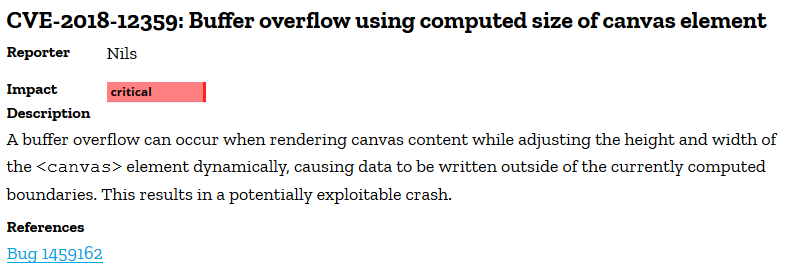
\includegraphics[width=\textwidth]{img/mfsa_example.png}
	\caption{Beispieleintrag auf der Mozilla Foundation Security Advisories Webseite}
	\label{fig:mfsa}
\end{figure}

% Infos über Sicherheitslücken: Alves et al: Projektspezifische Security Advisores und CVEDetails, Bugtracker
% Chowdhury und Zulkernine: Mozilla Foundation Security Advisores
% Vorverarbeitung abhängig von Art der Entitäten, die analysiert werden sollen: Nur Files? Einfach! Klassen, Methoden? Parsing-Schritt notwendig
% Alves et. al vergleichen mehrere Projekte: 1 C++ und 4 C Projekte -> Behandeln Unions und Structs wie Klassen!!! WTF! Vergleichbarkeit fragwürdig
% Außerdem: Alves et. al vergleichen immer 2 Commits nachheinander (der Commit, der Bug fixed und den direkt davor). Mehrere Commits pro Bug sind denkbar, was wenn letzter nur Typo fixed?
